% Этот шаблон документа разработан в 2014 году
% Данилом Фёдоровых (danil@fedorovykh.ru) 
% для использования в курсе 
% <<Документы и презентации в \LaTeX>>, записанном НИУ ВШЭ
% для Coursera.org: http://coursera.org/course/latex .
% Исходная версия шаблона --- 
% https://www.writelatex.com/coursera/latex/3.2

\documentclass[a4paper,12pt]{article}

%%% Работа с русским языком
\usepackage{cmap}					% поиск в PDF
\usepackage{mathtext} 				% русские буквы в формулах
\usepackage[T2A]{fontenc}			% кодировка
\usepackage[utf8]{inputenc}			% кодировка исходного текста
\usepackage[english,russian]{babel}	% локализация и переносы

%%% Дополнительная работа с математикой
\usepackage{amsmath,amsfonts,amssymb,amsthm,mathtools} % AMS
\usepackage{icomma} % "Умная" запятая: $0,2$ --- число, $0, 2$ --- перечисление

%% Номера формул
%\mathtoolsset{showonlyrefs=true} % Показывать номера только у тех формул, на которые есть \eqref{} в тексте.
%\usepackage{leqno} % Нумерация формул слева

%% Свои команды
\DeclareMathOperator{\sgn}{\mathop{sgn}}

%% Перенос знаков в формулах (по Львовскому)
\newcommand*{\hm}[1]{#1\nobreak\discretionary{}
	{\hbox{$\mathsurround=0pt #1$}}{}}

%%% Работа с картинками
\usepackage{graphicx}  % Для вставки рисунков
\graphicspath{{images/}{images2/}}  % папки с картинками
\setlength\fboxsep{3pt} % Отступ рамки \fbox{} от рисунка
\setlength\fboxrule{1pt} % Толщина линий рамки \fbox{}
\usepackage{wrapfig} % Обтекание рисунков текстом

%%% Работа с таблицами
\usepackage{array,tabularx,tabulary,booktabs} % Дополнительная работа с таблицами
\usepackage{longtable}  % Длинные таблицы
\usepackage{multirow} % Слияние строк в таблице

%%% Теоремы
\theoremstyle{plain} % Это стиль по умолчанию, его можно не переопределять.
\newtheorem{theorem}{Теорема}[section]
\newtheorem{proposition}[theorem]{Утверждение}

\theoremstyle{definition} % "Определение"
\newtheorem{corollary}{Следствие}[theorem]
\newtheorem{problem}{Задача}[section]

\theoremstyle{remark} % "Примечание"
\newtheorem*{nonum}{Решение}

%%% Программирование
\usepackage{etoolbox} % логические операторы

%%% Страница
\usepackage{extsizes} % Возможность сделать 14-й шрифт
\usepackage{geometry} % Простой способ задавать поля
\geometry{top=25mm}
\geometry{bottom=35mm}
\geometry{left=35mm}
\geometry{right=20mm}
%

\usepackage{fancyhdr} % Колонтитулы
\pagestyle{fancy}
%\renewcommand{\headrulewidth}{0mm}  % Толщина линейки, отчеркивающей верхний колонтитул
%\lfoot{Нижний левый}
%\rfoot{Нижний правый}
%\rhead{}
%\chead{Верхний в центре}
%\lhead{}
% \cfoot{Нижний в центре} % По умолчанию здесь номер страницы

\usepackage{setspace} % Интерлиньяж
%\onehalfspacing % Интерлиньяж 1.5
%\doublespacing % Интерлиньяж 2
%\singlespacing % Интерлиньяж 1

\usepackage{lastpage} % Узнать, сколько всего страниц в документе.

\usepackage{soul} % Модификаторы начертания

\usepackage{indentfirst} % Красная строка

\usepackage{soulutf8} % Модификаторы начертания

%\usepackage{hyperref}
%\usepackage[usenames,dvipsnames,svgnames,table,rgb]{xcolor}
%\hypersetup{				% Гиперссылки
%	unicode=true,           % русские буквы в раздела PDF
%	pdftitle={Заголовок},   % Заголовок
%	pdfsubject={Тема},      % Тема
%	pdfcreator={Создатель}, % Создатель
%	pdfproducer={Производитель}, % Производитель
%	pdfkeywords={keyword1} {key2} {key3}, % Ключевые слова
%	colorlinks=true,       	% false: ссылки в рамках; true: цветные ссылки
%	linkcolor=red,          % внутренние ссылки
%	citecolor=green,        % на библиографию
%	filecolor=magenta,      % на файлы
%	urlcolor=cyan           % на URL
%}

%\renewcommand{\familydefault}{\sfdefault} % Начертание шрифта

\usepackage{multicol} % Несколько колонок

\author{\LaTeX{} в Вышке}
\title{3.2 Оформление документа в целом}
\date{\today}

\begin{document} % конец преамбулы, начало документа
	\thispagestyle{empty}
	\begin{center}
		\textit{Федеральное государственное автономное образовательное\\ учреждение высшего образования }
		\vspace{0.5ex}
		
		\textbf{«Московский физико-технический институт\\ (национальный исследовательский университет)»}
	\end{center}
	\vspace{10ex}
	%\begin{flushright}
	%	\noindent
	%	\textit{Фамилия Имя Отчество}
	%	\\
	%	\textit{студент факультета экономики \\(группа 211И)}
	%\end{flushright}
	\begin{center}
		\vspace{13ex}
		\so{\textbf{Лабораторная работа №2.2.6}}
		\vspace{1ex}
		
		по курсу общей физики
		
		
		на тему:
		
		\textbf{\textit{<<Определение энергии активации\\ по температурной зависимости вязкости жидкости>>}}
		\vspace{30ex}
		\begin{flushright}
			\noindent
			\textit{Работу выполнил:}
			\\
			\textit{Баринов Леонид \\(группа Б02-827)}
		\end{flushright}
		\vfill
		Долгопрудный \\2019 год
	\end{center}
	\newpage
	\setcounter{page}{1}
	\section{Аннотация}
	В работе будет измерена скорость падения шариков при разной температуре жидкости. Будет вычислена вязкость жидкости по закону Стокса и расчитана энергии активации.
	\section{Теоритические сведения}
	В жидкостях, как и в кристаллах, каждая молекула находится в потенциальной яме электрического поля, создаваемого окружающими молекулами. Молекулы колеблются со средней частотой, близкой к частоте колебаний атомов в кристаллических телах ($\sim 10^{12}\ \text{Гц}$), и с амплитудой, определяемой размерами объема, предоставленного ей соседними молекулами. Глубина потенциальной ямы жидкостях больше средней кинетической энергии колеблющейся молекулы, поэтому молекулы колеблются вокруг более или менее стабильных положений равновесия. Однако у жидкостей различие между этими двумя энергиями невелико, так что молекулы нередко выскакивают из <<своей>> потенциальной ямы и занимают место в другой.
	
	Для того чтобы перейти в новое состояние, молекула должна преодолеть участки с большой потенциальной энергией, превышающей среднюю тепловую энергию молекул. Для этого тепловая энергия молекул должна — вследствие флуктуации — увеличиться на некоторую величину $W$, называемую энергией активации. Вследствие этого переходы молекул из одного положения равновесия в другое происходят сравнительно редко и тем реже, чем больше энергия активации.
	
	Отмеченный характер движения молекул объясняет как медленность диффузии в жидкостях, так и большую (по сравнению с газами) их вязкость. В газах вязкость объясняется происходящим при тепловом движении молекул переносом количества направленного движения. В жидкостях такие переходы существенно замедлены. Количество молекул, имеющих энергии больше $W$, в соответствии с формулой Больцмана экспоненциально зависит от $W$. Температурная зависимость вязкости жидкости выражается формулой (1):
	\begin{equation}
	\eta = Ae^{W/kT}
	\end{equation}
	
	Из формулы (1) следует, что вязкость жидкости при повышении температуры должна резко уменьшаться. Если отложить на графике логарифм вязкости $\ln \eta$ в зависимости от $1/Т$, то согласно (1) должна получиться прямая линия, по угловому коэффициенту которой можно определить энергию активации молекулы $W$ исследуемой жидкости. 
	
	Сила сопротивления, действующая при ламинарном обтекании шарика безграничной жидкостью (Закон Стокса):
	\begin{equation}
	F = 6\pi \eta r \upsilon 
	\end{equation}
	где $\eta$ -- вязкость жидкости, $\upsilon$ -- скорость шарика, $r$ -- его радиус.
	
	Уравнение движения шарика в жидкости:
	\begin{equation}
	\upsilon(t) = \upsilon_{\text{уст}} - [\upsilon_{\text{уст}} - \upsilon(0)]e^{-t/\tau}
	\end{equation}
	$\upsilon(0)$ -- скорость шарика в момент начала его движения в жидкости
	\begin{equation}
	\upsilon_{\text{уст}} = \frac{2}{9}gr^2\frac{\rho-\rho_{\text{ж}}}{\eta} 
	\end{equation}
	\[\tau = \frac{2}{9}\frac{r^2 \rho}{\eta}  \]
	Как видно из (3), скорость шарика экспоненциально приближается к установившейся скорости $\upsilon_{\text{уст}}$. Установление скорости определяется величиной $\tau$, имеющей размерность времени и называющейся временем релаксации.
	
	Измеряя на опыте установившуюся скорость падения шариков $\upsilon_{\text{уст}}$ и величины $r, \rho, \rho_{\text{ж}}$, можно определить вязкость жидкости по формуле, следующей из (4):
	\begin{equation}
	 \eta = \frac{2}{9}gr^2\frac{\rho-\rho_{\text{ж}}}{\upsilon_{\text{уст}}} 
	\end{equation}
	Характер обтекания определяется значением числа Рейнольдса 
	\begin{equation}
	\text{Re} = \frac{\upsilon r \rho_{\text{ж}}}{\eta}
	\end{equation}
	Путь $S$ может быть найден посредством интегрирования (3). $\upsilon(0) = 0$
	\begin{equation}
	S = \upsilon_{\text{уст}}\tau\left(\frac{t}{\tau} - 1 + e^{-t/\tau}\right)
	\end{equation}
	Из формулы (7) легко видеть, что $S\gg\tau\upsilon_{\text{уст}}$ при $t\gg\tau$
	
	После неравенство определяет допустимое расстояние между границей жидкости и верхней меткой.
	\section{Оборудование}
	В работе используются: стеклянный цилиндр с исследуемой жидкостью (глицерин); термостат; секундомер; горизонтальный компаратор; микроскоп; мелкие шарики (диаметром около $1\text{мм}$)
	\subsection{Экспериментальная установка}
	\begin{figure}[h]
		\begin{center}
			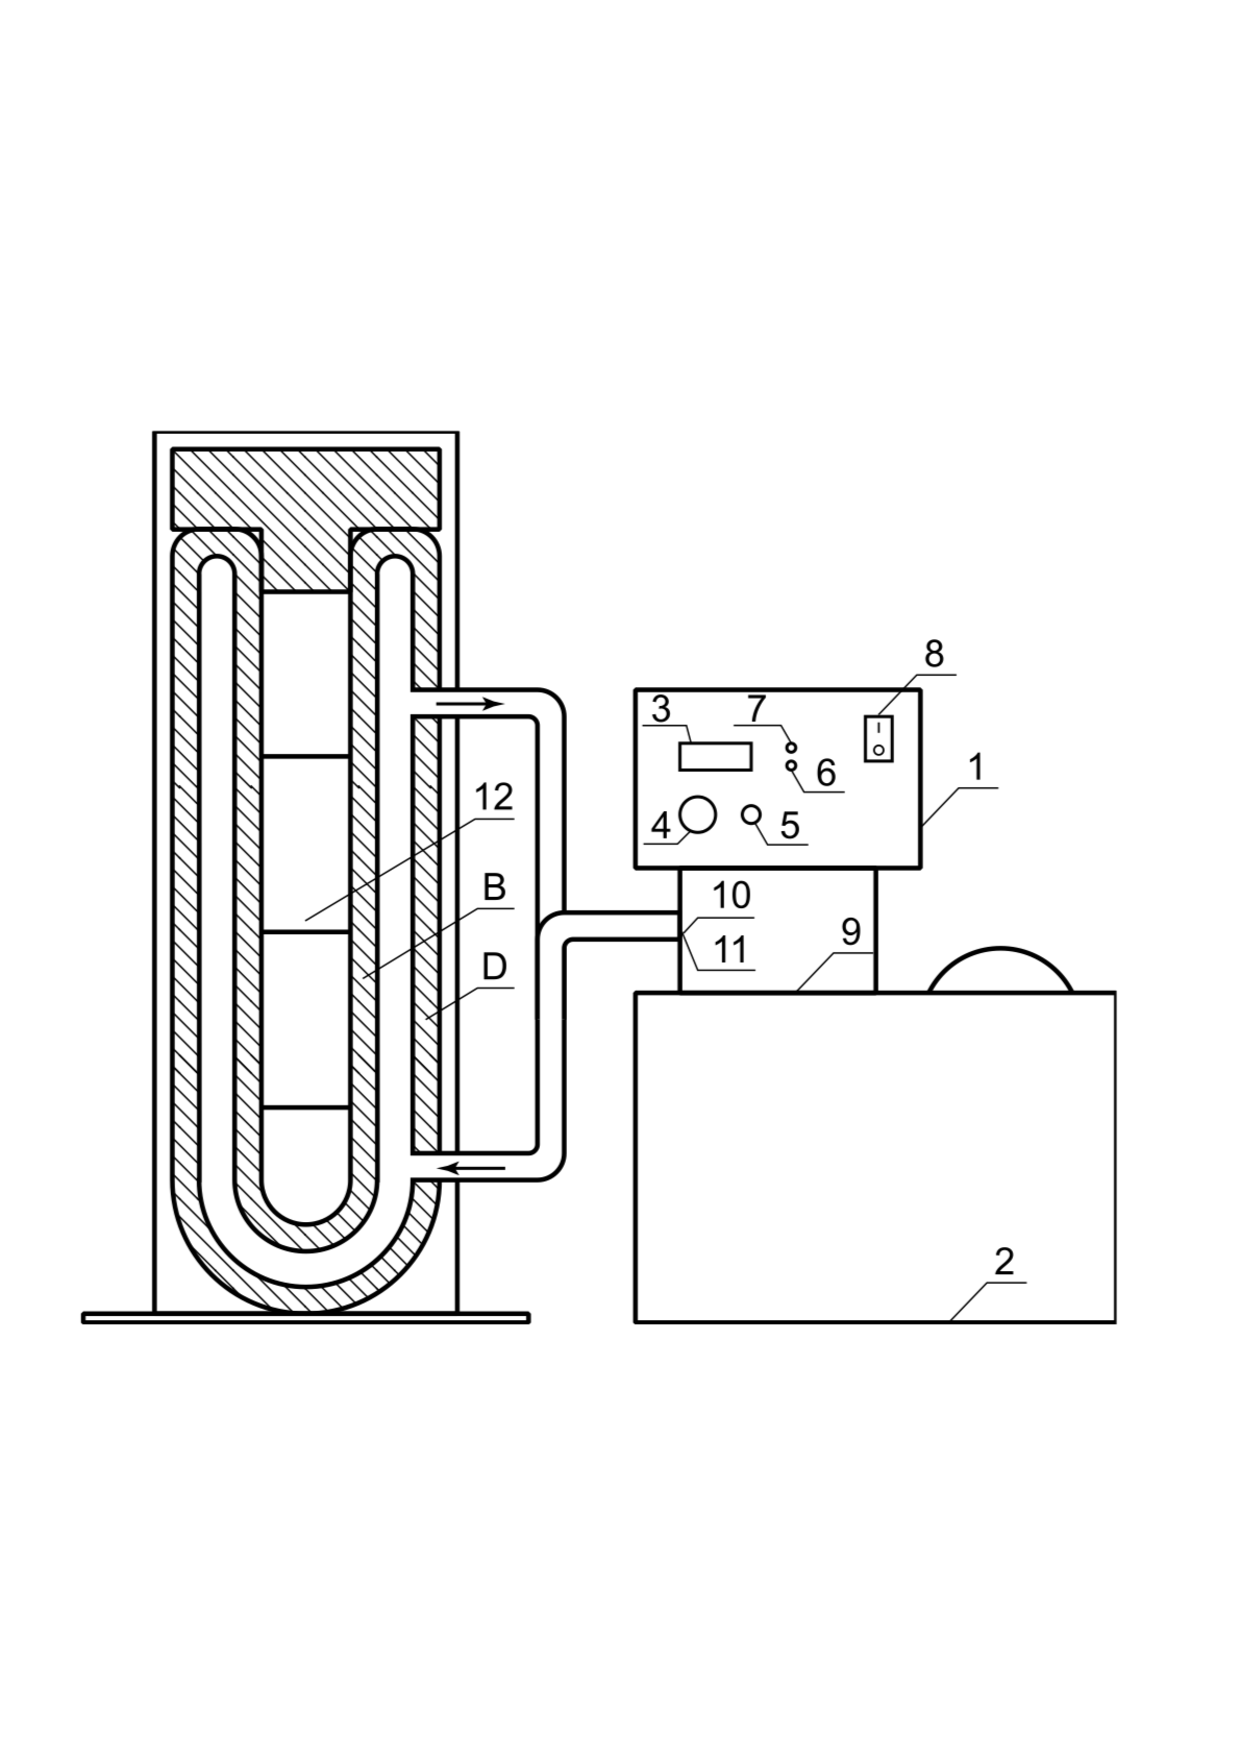
\includegraphics[width=0.5\linewidth]{1}
		\end{center}
	\caption{Установка для определения коэффициента вязкости жидкости}
	\end{figure}
\begin{enumerate}
	\item блок терморегулирования
	\item ванна
	\item индикаторное табло
	\item ручка установки температуры
	\item кнопка переключения режимов установки/контроля температуры
	\item индикатор уровня жидкости
	\item индикатор включения нагревателя
	\item сетевой выключатель прибора
	\item крышка
	\item входной и выходной патрубки насоса
	\item входной и выходной патрубки теплообменника (вода из водопровода)
	\item температура жидкости (равна температуре воды в термостате).
\end{enumerate}
Сосуд B помещен в рубашку D
\subsection{Микроскоп}
Радиусы шариков измеряются горизонтальным компаратором или микроскопом. Плотность шариков $\rho$ определяется из таблиц 
\[\rho_{\text{стекла}} = 2,5\text{г}/\text{см}^3\]
\[\rho_{\text{стали}} = 7,8\text{г}/\text{см}^3\]
 Плотность исследуемой жидкости определяется по графику $\rho_{\text{ж}}(Т)$, Рис. 2.
 \begin{figure}[!h]
 	\begin{center}
 		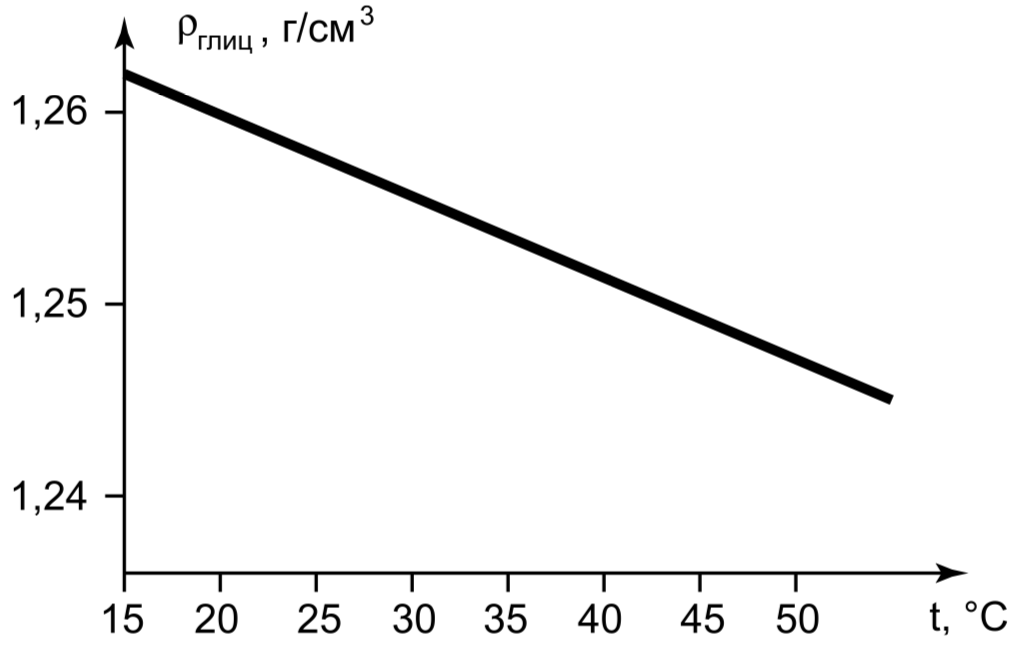
\includegraphics[width=0.5\linewidth]{2}
 	\end{center}\
 	\caption{Зависимость плотности глицерина от температуры}
 \end{figure}

\section{Результаты измерений и обработка результатов}
\noindent Выберем 10 стеклянных и 10 стальных шариков. Измерим их радиусы.

Измерьте установившиеся скорости падения шариков и вычислите вязкость $\eta$ по формуле (5). Измерения выполним для 4-5 значений температуры в интервале от комнатной до $50-60^\circ C$. Результаты занесем в Таблицу 1. Время измеряется при прохождением шарика расстояния $l = 0,1 \text{м}$
\begin{table}[!h]
	\begin{center}
	\begin{tabular}{|c|c|c|c|c|c|}
		\hline
		$T, ^\circ\! C$  & $d, \text{мм}$    & $t, \text{с}$   & $\upsilon_{\text{уст}}, \text{мм}/\text{с}$    & $\eta, 10^{-3} \ \text{Па}\cdot \text{с}$   & $\Delta\eta, 10^{-3} \ \text{Па}\cdot \text{с}$\\ \hline
		\multicolumn{6}{|c|}{Стеклянные шарики}    \\ \hline
		\multirow{2}{*}{22,9} & 1,8  & 36,67 & 2,73  & 802  & 16 \\ \cline{2-6}
		& 1,9  & 35,65 & 2,81  & 869  & 16 \\ \hline
		\multirow{2}{*}{30,1} & 1,8  & 27,13 & 3,69  & 593  & 12 \\ \cline{2-6}
		& 1,9  & 24,86 & 4,02  & 606  & 12 \\ \hline
		\multirow{2}{*}{38,1} & 1,8  & 14,08 & 7,10  & 310  & 7  \\  \cline{2-6}
		& 1,9  & 13,68 & 7,31  & 336  & 8  \\ \hline
		\multirow{2}{*}{46}   & 1,8  & 7,51  & 13,32 & 166  & 5  \\  \cline{2-6}
		& 1,9  & 7,21  & 13,87 & 177  & 6  \\ \hline
		\multirow{2}{*}{55}   & 2    & 4,93  & 20,28 & 134  & 6  \\  \cline{2-6}
		& 2    & 4,63  & 21,60 & 126  & 6  \\ \hline
		\multicolumn{6}{|c|}{Стальные шарики}    \\ \hline
		\multirow{2}{*}{22,9} & 0,8  & 38,49 & 2,60  & 877  & 78 \\  \cline{2-6}
		& 0,8  & 46,68 & 2,14  & 1064 & 95 \\ \hline
		\multirow{2}{*}{30,1}& 0,8  & 29,25 & 3,42  & 667  & 59 \\  \cline{2-6}
		& 0,75 & 23,35 & 4,28  & 468  & 45 \\ \hline
		\multirow{2}{*}{38,1} & 0,85 & 11,71 & 8,54  & 302  & 26 \\  \cline{2-6}
		& 0,85 & 14,25 & 7,02  & 367  & 31 \\ \hline
		\multirow{2}{*}{46}   & 0,75 & 9     & 11,11 & 181  & 18 \\  \cline{2-6}
		& 0,9  & 7,01  & 14,27 & 202  & 17 \\ \hline
		\multirow{2}{*}{55}   & 0,75 & 5,67  & 17,64 & 114  & 12 \\  \cline{2-6}
		& 0,8  & 4,28  & 23,36 & 98   & 10 \\ \hline
	\end{tabular}
\end{center}
\caption{Определение вязкости глицерина}
\end{table}

Для каждого из опытов вычислим значение числа Рейнольдса Re, оценим время релаксации $\tau$ (по формуле (4)) и путь релаксации S. Результаты занесем в Таблицу 2. Усредним значения вязкости. Результат занесем в Таблицу 3.

\begin{table}[h]
	\begin{center}
	\begin{tabular}{|c|c|c|c|c|c|}
		\hline
		$T, ^\circ\! C$  & $d, \text{мм}$   & $\upsilon_{\text{уст}}, \text{мм}/\text{с}$    & Re    & $\tau, \text{мс}$  & $S, \text{мкм}$   \\ \hline
		\multicolumn{6}{|c|}{Стеклянные шарики}    \\ \hline
		\multirow{2}{*}{22,9} & 1,8  & 2,73  & 0,004 & 0,56 & 1,53  \\ \cline{2-6}
		& 1,9  & 2,81  & 0,004 & 0,58 & 1,62  \\ \hline
		\multirow{2}{*}{30,1} & 1,8  & 3,69  & 0,007 & 0,76 & 2,80  \\ \cline{2-6}
		& 1,9  & 4,02  & 0,008 & 0,83 & 3,33  \\ \hline
		\multirow{2}{*}{38,1} & 1,8  & 7,10  & 0,026 & 1,45 & 10,29 \\ \cline{2-6}
		& 1,9  & 7,31  & 0,026 & 1,49 & 10,91 \\ \hline
		\multirow{2}{*}{46}   & 1,8  & 13,32 & 0,091 & 2,72 & 36,18 \\ \cline{2-6}
		& 1,9  & 13,87 & 0,094 & 2,83 & 39,26 \\ \hline
		\multirow{2}{*}{55}   & 2    & 20,28 & 0,190 & 4,14 & 83,97 \\ \cline{2-6}
		& 2    & 21,60 & 0,216 & 4,41 & 95,20 \\ \hline
		\multicolumn{6}{|c|}{Стальные шарики}    \\ \hline
		\multirow{2}{*}{22,9}& 0,8  & 2,60  & 0,001 & 0,32 & 0,82  \\ \cline{2-6}
		& 0,8  & 2,14  & 0,001 & 0,26 & 0,56  \\ \hline
		\multirow{2}{*}{30,1} & 0,8  & 3,42  & 0,003 & 0,42 & 1,42  \\ \cline{2-6}
		& 0,75 & 4,28  & 0,004 & 0,52 & 2,23  \\ \hline
		\multirow{2}{*}{38,1} & 0,85 & 8,54  & 0,015 & 1,04 & 8,86  \\ \cline{2-6}
		& 0,85 & 7,02  & 0,010 & 0,85 & 5,98  \\ \hline
		\multirow{2}{*}{46}     & 0,75 & 11,11 & 0,029 & 1,35 & 15,00 \\ \cline{2-6}
		& 0,9  & 14,27 & 0,040 & 1,73 & 24,73 \\ \hline
		\multirow{2}{*}{55}    & 0,75 & 17,64 & 0,073 & 2,14 & 37,80 \\ \cline{2-6}
		& 0,8  & 23,36 & 0,121 & 2,84 & 66,33 \\ \hline
	\end{tabular}
\end{center}
\caption{Значение числа Рейнольдса Re, времени релаксации $\tau$, пути релаксации $S$}
\end{table}

\begin{table}[h]
	\begin{center}
	\begin{tabular}{|c|c|c|c|c|}
		\hline
		$T, \text{K}$   & $\eta, 10^{-3} \ \text{Па}\cdot \text{с}$ & $\sigma_\text{сл}, \ \text{Па}\cdot \text{с}$    & $\sigma_\text{сист}, \ \text{Па}\cdot \text{с}$     & $\sigma_\eta, \text{Па}\cdot \text{с}$  \\ \hline
		295,9 & 902,96 & 97,29 & 116,34 & 151,66 \\ \hline
		303,1 & 583,38 & 72,31 & 77,85  & 106,25 \\ \hline
		311,1 & 328,85 & 25,47 & 41,09  & 48,34  \\ \hline
		319   & 181,44 & 13,35 & 24,82  & 28,19  \\ \hline
		328   & 117,92 & 13,77 & 18,43  & 23,01  \\ \hline
	\end{tabular}
\end{center}
\caption{Зависимость вязкости глицерина $\eta$ от температуры $T$}
\end{table}

Построим график зависимости $\ln\eta$ от $1/T$ по результатам в Таблице 4.

\begin{table}[h]
	\begin{center}
	\begin{tabular}{|c|c|c|}
		\hline
		$\ln\eta, \ \text{Па}\cdot \text{с}$   & $\Delta \ln\eta, \ \text{Па}\cdot \text{с}$   & $1/T, \text{мК},{-1}$  \\ \hline
		6,81 & 0,168 & 3,38 \\ \hline
		6,37 & 0,182 & 3,30 \\ \hline
		5,80 & 0,147 & 3,21 \\ \hline
		5,20 & 0,155 & 3,13 \\ \hline
		4,77 & 0,195 & 3,05 \\ \hline
	\end{tabular}
\end{center}
\caption{Данные для построения графика}
\end{table}

 \begin{figure}[!h]
	\begin{center}
		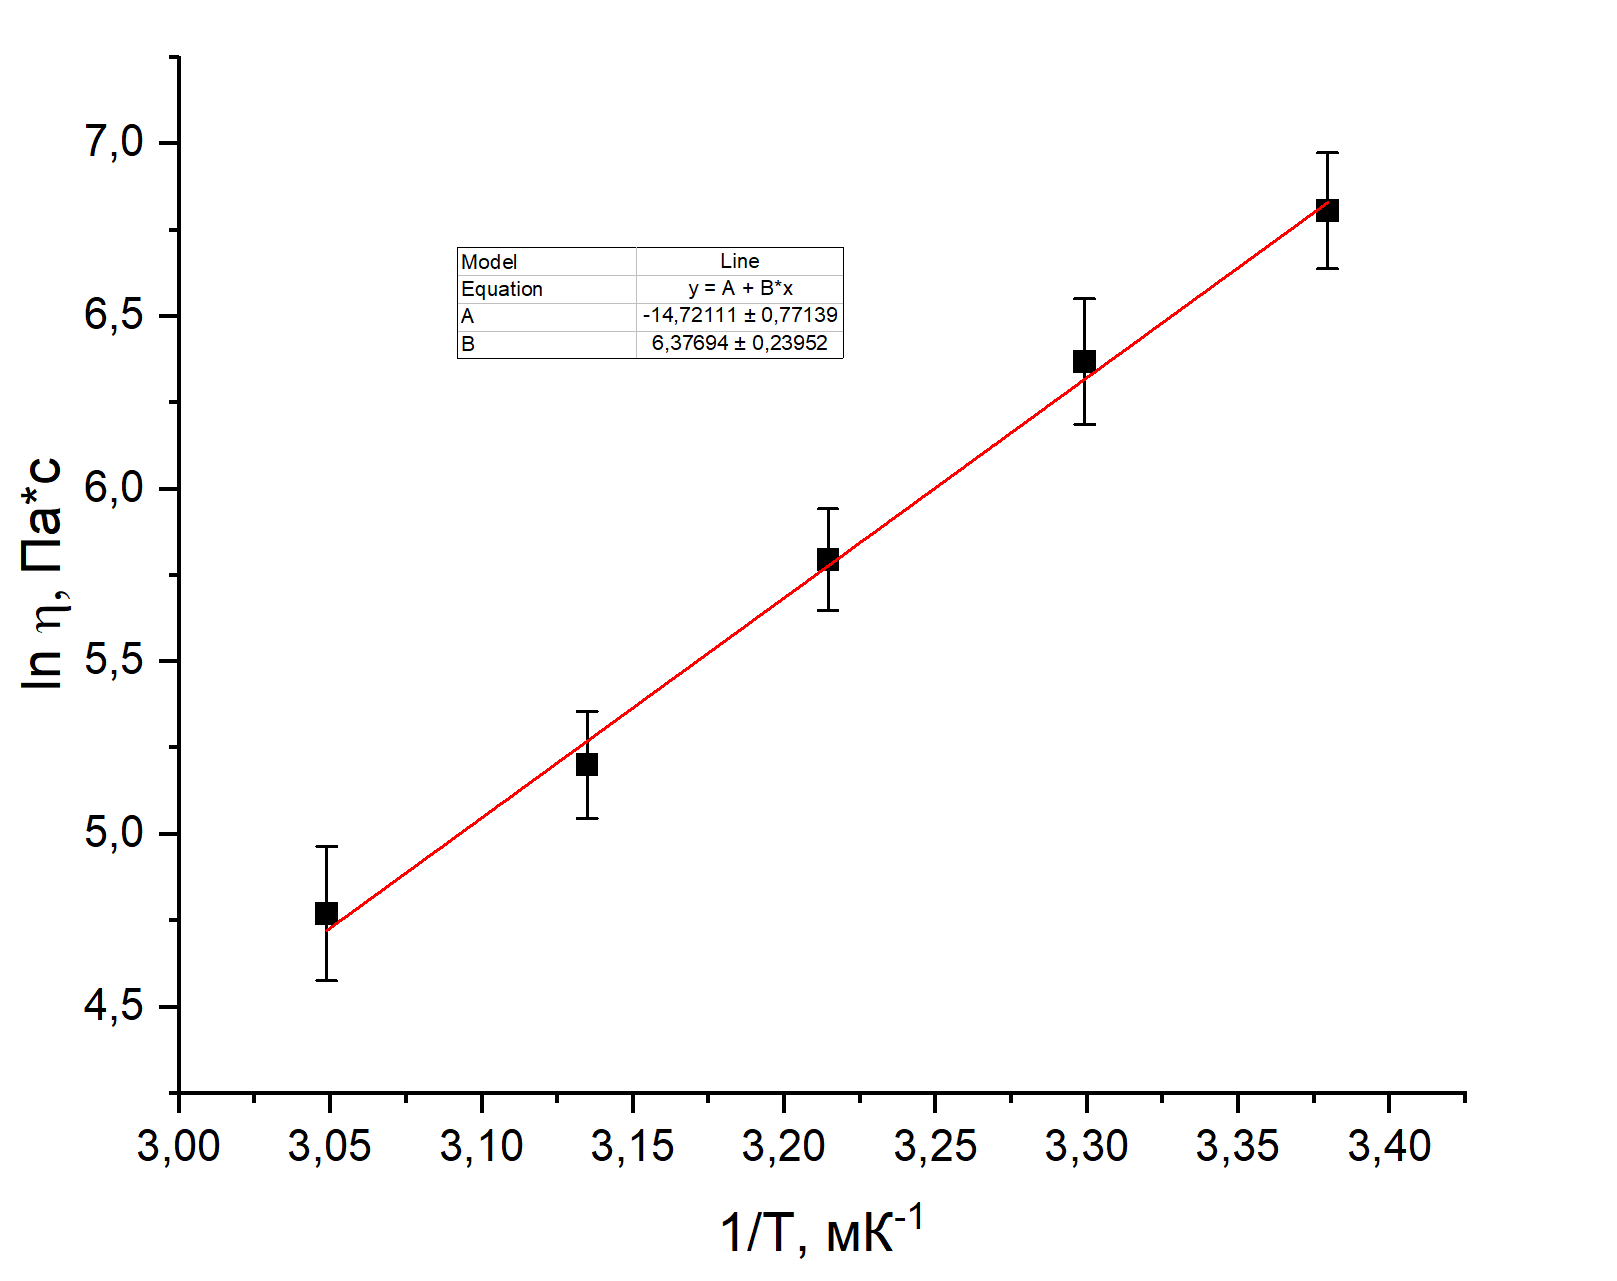
\includegraphics[width=0.7\linewidth]{3}
	\end{center}\
	\caption{Зависимость логарифма вязкости $ln \eta$ от величины, обратной температуре глицерина $1/T$ }
\end{figure}

Из графика получаем:
\[W = (0,88\pm0,03)\cdot 10^{-19} \text{Дж} \]
\[W = (0,55\pm0,02)\text{эВ}\]

\section{Обсуждение результатов и выводы}
В работе было поведение вычисление вязкости глицерина $\eta$ для каждого шарика при заданной температуре. (Таблица 1)

Для каждого из опытов было вычислено значение числа Рейнольдса Re (Таблица 2). $Re<0,5$, что свидетельствует о ламинарном характере обтекания шариков жидкостью. 

Была проведена оценка времени релаксации $\tau$ и пути релаксации $S$. Значение оказалась малы по сравнению со значением пути и времени при измерениях установившийся скоростью, что в данном эксперименте было возможно применение формулы Стокса.

Было получено усредненное значение вязкости жидкости для каждой из измеряемых температур. (Таблица 3). Данные в пределах погрешности совпадают с табличными.

По графику зависимости логарифма вязкости $ln \eta$ от величины, обратной температуре глицерина $1/T$ было получено значение энергии активации молекул глицерина:
\[W = (0,88\pm0,03)\cdot 10^{-19} \text{Дж} \]
\[W = (0,55\pm0,02)\ \text{эВ}\]
Экспериментальные данные совпадают с табличными. ($W = 0,54\text{эВ}$)
	
	
\end{document}